\section{Introduction}

The goal of this project is to expand the capabilities of the solution for the previous part with a "real" network layer. For hosts this means a layer implementation that can send and receive datagrams with messages from/to the transport layer. For the routers, this means a layer implementation that can receive datagrams and forward them in the direction of the destination host.\\
Figure \ref{fig:GivenTopology} from the project description illustrates the topology for which it is a requirement that the solution functions. Note that the routers are called 1 and 2 rather than C and D, both in the source code and this report, to ease distinction between routers and hosts.

\begin{figure}[H]
\centering
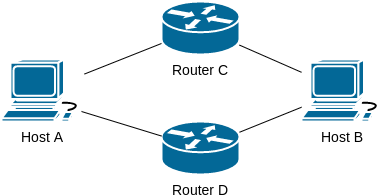
\includegraphics[width=0.5\textwidth]{../figs/network-topology.png}
\caption{Topology for which it is required that the implementation functions}
\label{fig:GivenTopology}
\end{figure}



\subsection{Terms}
The following are additional terms used as shorthands:
\begin{itemize}
\item LL: Link Layer
\item NL: Network Layer
\item TL: Transport Layer
\end{itemize}



